\subsection{Le processus d'importation d'un fichier}

Dans cette sous-section, nous suivrons le destin d'un fichier pendant son importation, depuis son arrivée à l'API dans le corps d'une requête POST, jusqu'à l'enregistrement de ses données dans la table appropriée de la base de données adéquate. Nous utiliserons à titre d'exemple un fichier LCCC (La Compagnie des Cartes Carburant SAS) qui est un type de fichier de transactions de carburant au format \Verb|csv| (Figure~\ref{fig:lccc}).

\begin{figure}[ht]
    \centering
    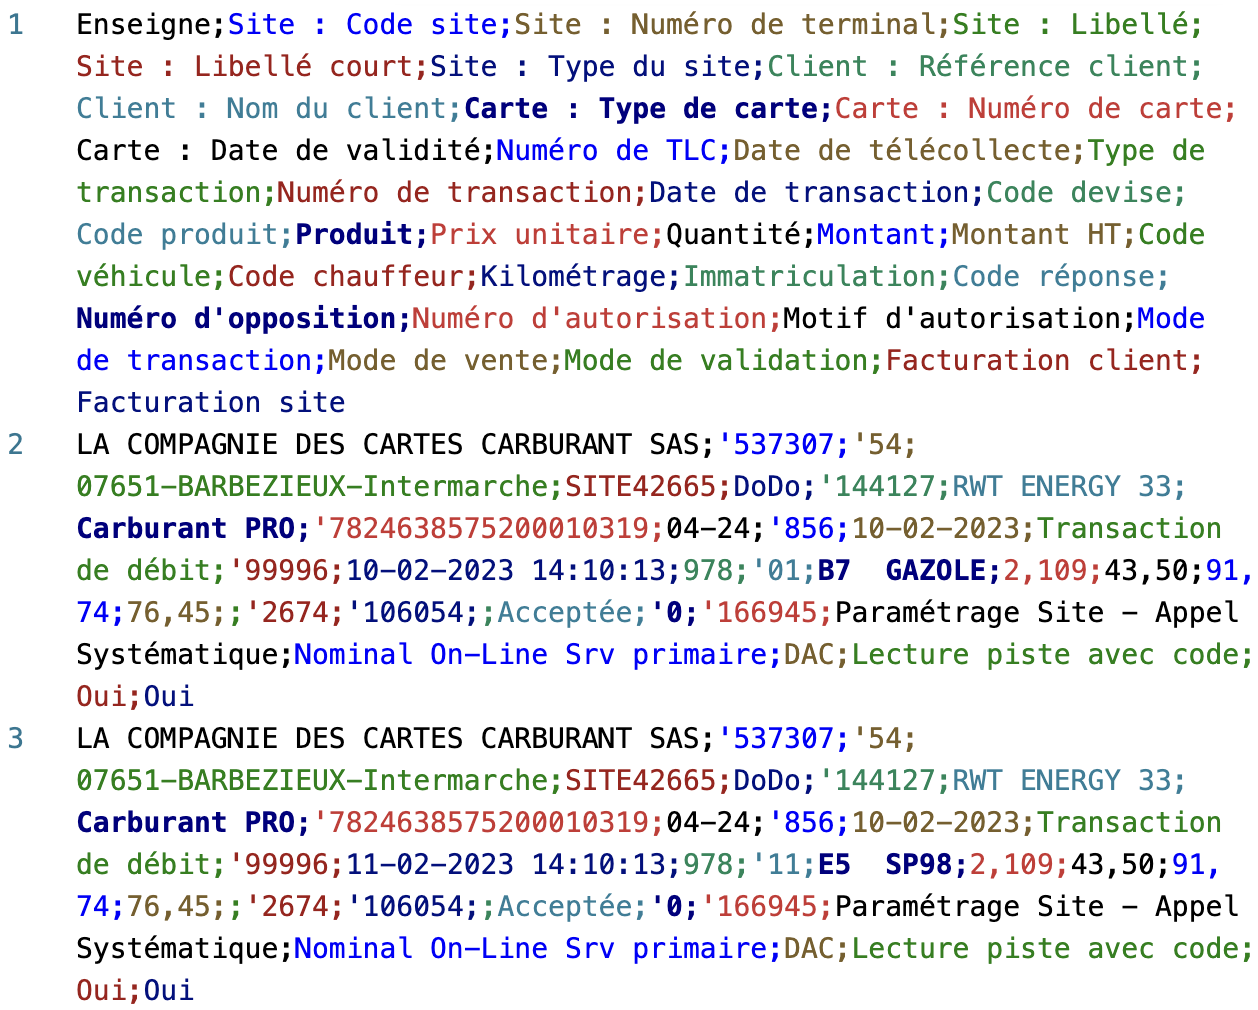
\includegraphics[width=\textwidth]{img/lccc-csv}
    \caption{Exemple d'un fichier LCCC.}
    \label{fig:lccc}
\end{figure}

Pour l'API, il est possible d'envoyer des fichiers dans le corps d'une requête POST au format encodé en base64, en tant que partie d'un objet JSON bien défini, comme démontré dans le Code source~\ref{code:lccc-payload}. Cette charge utile est validée avant d'être acceptée par l'API, plus précisément l'application Laravel utilise la méthode \Verb|rules()| de la classe \Verb|UploadStoreRequest| créée par nous pour la valider (Code source~\ref{code:upload-store-request}).

Cette classe se trouve dans le dossier \Verb|app/Http/Requests|. Elle étend la classe \Verb|FormRequest| de Laravel, permettant ainsi de définir les règles de validation pour la requête de stockage (store request) d'import de fichiers.

La méthode \Verb|rules()| définit les règles de validation pour les différentes parties de la requête. Les règles sont définies sous forme d'un tableau associatif. Parmi les règles définies :

\begin{itemize}
    \item Le champ \Verb|client_app| doit être présent, être un nombre entier et être une des valeurs autorisées spécifiées dans la configuration du projet (\Verb|allowed_client_app|).
    \item Le champ \Verb|parameters| doit être un tableau avec au moins deux éléments.
    \item Les éléments spécifiques du champ \Verb|parameters| (\Verb|client_id| et \Verb|user_id|) doivent être présents, être des nombres entiers et être obligatoires.
    \item Le champ \Verb|files| doit être un tableau avec au moins un élément.\footnote{Pour l'instant, l'API n'est pas en mesure de gérer plus d'un fichier. Si plusieurs fichiers sont présents dans la charge utile, ils ne sont pas pris en compte.}
    \item Les éléments spécifiques du champ \Verb|files| (\Verb|content|) doivent être présents, commencer par \Verb|data:text/plain;base64,| et avoir une longueur minimale de 27 caractères.
\end{itemize}

En somme, la classe \Verb|UploadStoreRequest| sert de mécanisme de validation pour les requêtes POST envoyées à l'API, en s'assurant que les données fournies sont conformes aux règles spécifiées, contribuant ainsi à la sécurité et à la cohérence des données entrantes.

La charge utile doit être envoyée à la route appropriée définie dans le fichier \Verb|routes/api.php| (Code source~\ref{code:file-import-route}).

\begin{code}
    \caption{La charge utile (payload) à envoyer contenant le fichier encodé au format base64 et certaines métadonnées associées.}
    \inputminted[samepage]{json}{code/lccc-payload.json}
    \label{code:lccc-payload}
\end{code}

\begin{code}
    \caption{La définition de la route d'importation de fichiers dans le fichier \Verb{routes/api.php}.}
    \inputminted[firstline=47,lastline=47]{php}{code/api.php}
    \label{code:file-import-route}
\end{code}

Cette route est définie pour une requête POST vers l'URL \Verb|/command/uploads/{category}/{type}|. Lorsqu'une requête POST est effectuée vers cette URL, elle sera traitée par la méthode \Verb|upload| du contrôleur \Verb|UploadController|. Cette méthode prendra en charge le traitement de la requête et la gestion de l'importation des fichiers correspondant à la catégorie et au type spécifiés dans l'URL. Dans le cas de notre fichier, la catégorie est \Verb|fuel-transactions|, le type est \Verb|lccc|. Cette définition de route établit une correspondance entre une URL POST spécifique et la méthode du contrôleur qui gère le traitement de la requête et les opérations nécessaires. Cela permet de créer une API RESTful qui répond aux requêtes POST adressées à cette URL particulière.

\begin{code}
    \caption{La classe \Verb{UploadStoreRequest}.}
    \inputminted{php}{code/UploadStoreRequest.php}
    \label{code:upload-store-request}
\end{code}

\subsubsection{La méthode \Verb{upload} de la classe \Verb{UploadController}}

La classe \Verb|UploadController| (Code source~\ref{code:upload-controller}) représente une classe de contrôleur dans le projet. Elle gère les requêtes en répondant à certaines routes définies dans l'API. Nous ne nous occupons ici que de la route d'importation des fichiers et de la méthode \Verb{upload} de la classe. Lorsqu'une requête POST est effectuée vers cette route, la méthode \Verb{upload} du contrôleur est appelée.

\begin{code}
    \caption{La version simplifiée de la classe \Verb{UploadController}.}
    \inputminted{php}{code/UploadController.php}
    \label{code:upload-controller}
\end{code}

La méthode \Verb{upload} prend trois paramètres : une instance de la classe \Verb{UploadStoreRequest} (Code source~\ref{code:upload-store-request}, page~\pageref{code:upload-store-request}) pour la validation de la requête, une chaîne \Verb{category} pour la catégorie du fichier et une chaîne \Verb{type} pour le type de fichier. La méthode utilise ensuite la classe \Verb{Artisan} pour appeler une commande Artisan personnalisée correspondant à l'importation du fichier en utilisant la catégorie et le type spécifiés. Les paramètres tels que le jeton d'autorisation, les données validées de la requête et les détails de la catégorie et du type sont transmis à la commande.

Après l'exécution de la commande, la sortie est récupérée et analysée en tant que JSON. Cette sortie représente le résultat de l'importation du fichier, qui est ensuite renvoyé sous forme de réponse JSON avec le code de statut 201 (Créé). En somme, la classe \Verb{UploadController} agit comme un pont entre les requêtes d'importation de fichiers, la validation des données et l'exécution de la commande associée pour traiter les fichiers importés et renvoyer les résultats appropriés.
\subsubsection{La classe abstraite \Verb{UploadTrigger} et ses enfants}

Dans l'API, les commandes Artisan personnalisées qui sont appelées par la méthode \Verb|upload| de la classe \Verb|UploadController| sont représentées par la classe abstraite \Verb|UploadTrigger| et ses enfants. Elles se trouvent dans le dossier \Verb|app/Console/Commands| du projet.

La classe \Verb|UploadTrigger| est une classe de commande, destinée à gérer le processus de déclenchement d'une importation de fichiers. Elle étend la classe \Verb|Command| de Laravel, fournissant ainsi la base pour définir des commandes spécifiques.

La classe contient des propriétés statiques \Verb|storageDirectory| et \Verb|workDirectory| pour les répertoires de stockage et de travail. Dans le constructeur (Code source~\ref{code:upload-trigger-constructor}), des arguments d'entrée (\Verb|input|, \Verb|token|, \Verb|category| et \Verb|type|) sont définis pour la commande, ainsi qu'une définition d'entrée pour les utiliser.

\begin{code}
    \caption{Le constructeur de la classe \Verb{UploadTrigger}.}
    \inputminted[firstline=28,lastline=38]{php}{code/UploadTrigger.php}
    \label{code:upload-trigger-constructor}
\end{code}

La méthode \Verb|handle()| (Code source~\ref{code:upload-trigger-handle}) est appelée lorsque la commande est exécutée. Elle enregistre un nouvel \Verb|Upload| en utilisant les paramètres fournis, puis déclenche un événement \Verb|StepStart| avec les paramètres nécessaires pour démarrer l'étape de traitement. Le statut de l'importation est mis à jour et les informations sont enregistrées dans un fichier journal.

\begin{code}
    \caption{La méthode \Verb{handle()} de la classe \Verb{UploadTrigger}.}
    \inputminted[firstline=40,lastline=62]{php}{code/UploadTrigger.php}
    \label{code:upload-trigger-handle}
\end{code}

La méthode \Verb|recordNewUpload()| (Code source~\ref{code:upload-trigger-record-new-upload}) enregistre les détails de l'importation dans la base de données, gère les fichiers associés et renvoie un objet \Verb|Upload|.

\begin{code}
    \caption{La méthode \Verb{recordNewUpload()} de la classe \Verb{UploadTrigger}.}
    \inputminted[firstline=65,lastline=88]{php}{code/UploadTrigger.php}
    \label{code:upload-trigger-record-new-upload}
\end{code}

La méthode \Verb|saveInDirectories()| (Code source~\ref{code:upload-trigger-save-in-directories}) gère l'enregistrement des fichiers dans les répertoires de stockage et de travail, tout en gérant les paramètres associés.

\begin{code}
    \caption{La méthode \Verb{saveInDirectories()} de la classe \Verb{UploadTrigger}.}
    \inputminted[firstline=90,lastline=121]{php}{code/UploadTrigger.php}
    \label{code:upload-trigger-save-in-directories}
\end{code}

L'objectif global de la classe est de gérer le flux de travail lié à l'importation de fichiers, de l'enregistrement initial à l'enregistrement des fichiers et à la mise à jour des statuts et des journaux correspondants. Cette classe de commande abstraite joue un rôle essentiel dans la gestion des processus d'importation de fichiers dans l'API, en encapsulant les étapes et les opérations associées dans des méthodes clés.

Cette classe contient les fonctionnalités communes des commandes d'importation de fichiers. Pour créer des commandes spécifiques à un fichier, il convient d'étendre cette classe et de définir les attributs spécifiques dans les classes enfants.

La classe \Verb|UploadTriggerLCCC| (Code source~\ref{code:upload-trigger-lccc}) est une classe de commande spécifique à notre fichier d'exemple, destinée à gérer le déclenchement de l'importation des transactions de carburant spécifiques à LCCC. Elle étend la classe abstraite \Verb|UploadTrigger|, héritant ainsi des fonctionnalités et du comportement définis dans la classe parente.

La propriété \Verb|signature| est définie pour cette commande, indiquant comment la commande doit être appelée à partir de la ligne de commande Laravel ou à partir du code, comme dans la méthode \Verb|upload| de la classe \Verb|UploadController|. Dans ce cas, la signature est \Verb|upload-fuel-transactions:lccc|.

La propriété \Verb|description| donne une brève description de ce que fait la commande. Dans ce cas, la description est \foreignquote{french}{Import fuel transactions LCCC}, ce qui indique clairement que la commande est utilisée pour l'importation des transactions de carburant spécifiques à LCCC.

\begin{code}
    \caption{La classe \Verb{UploadTriggerLCCC}.}
    \inputminted{php}{code/UploadTriggerLCCC.php}
    \label{code:upload-trigger-lccc}
\end{code}